% !TeX spellcheck = en_US
\chapter{Trajectory Planning}

\section{Introduction}

\subsection{Definitions}
\hlr{Goal:} compute a function of time that describes the motion of robot's joints. Depending on the task and time constraints, there will be different restrictions on the trajectory.
\begin{itemize}
	\item A {\color{blue} \textbf{Path}} is a set of points in the joint/operational space, as geometrical description of the motion
	\item A {\color{red} \textbf{Trajectory}} is a path through space as a function of time\\
	\textbf{{\color{red} \boxed{\text{Trajectory = Path + Time Law}}}}
\end{itemize}

\subsection{Joint space vs. Operational Space Trajectory Planning}
\begin{itemize}
	\item Joint space: planning is done in terms of joint positions, velocities and accelerations: ${\color{red} q, \dot{q}, \ddot{q}}$. $\Rightarrow$ trajectory of the \ac{ee} should NOT be important.
	\item Operational space: planning is done in terms of \ac{ee} positions, orientation and their derivatives: ${\color{blue} \textbf{x}_E, \dot{\textbf{x}}_E, \ddot{\textbf{x}}_E}$. This gives more control over the \ac{ee} path, \eg, for melding, gluing applications.
\end{itemize}

\begin{figure}[hbt!]
	\centering
	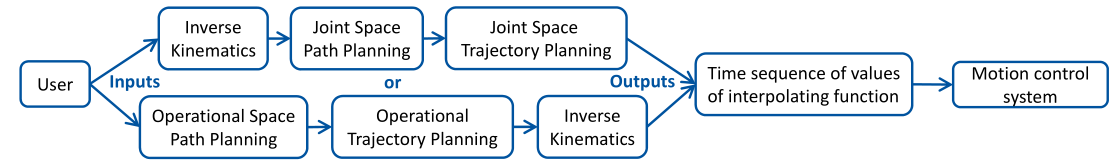
\includegraphics[width=\textwidth]{trajectory-planning.png}
	\caption{Trajectory planning procedure.}
	\label{fig:trajectory-planning}
\end{figure}
\begin{itemize}
	\item Inputs: path description, geometric / kinematic constraints (usually in operational space), constraints resulting from the manipulator dynamics
	\item Outputs: A time sequence of values for the joints' positions, velocities and accelerations as needed by the motion control system
	\item The paths and trajectories are not defined by the user explicitly in each point, but as a set of relevant \ac{param}: start, end points, possible intermediate points, geometric primitives, total time, maximum accelerations and velocities
\end{itemize}

\section{Joint Space Trajectories}
Given start and end \ac{ee} poses $\textbf{P}_{start}, \textbf{P}_{end}$ (and possible intermediate poses), apply inverse kinematics to get the joint poses (\figref{fig:trajectory-planning}).
\begin{equation*}
	\left. \begin{matrix*}[l]
		{\color{blue} \textbf{P}_{start}} \Rightarrow {\color{red} \textbf{q}(t_{start})}\\
		{\color{blue} \textbf{P}_{end}} \Rightarrow {\color{red} \textbf{q}(t_{end})}
	\end{matrix*} \right\} \Rightarrow {\color{red} \textbf{q}_t, \dot{\textbf{q}}_t, \ddot{\textbf{q}}_t} \quad\text{for}\quad t\in[t_{start}, t_{end}]
\end{equation*}

\subsection{Point-to-Point Motion}
Possible \hlb{timing laws} for point-to-point motion:
\begin{itemize}
	\item Cubic polynomial for the joints motion: can impose start, end positions and velocities
	\begin{align*}
		&q_i(t) = a_{i,3}t^3 + a_{i,2}t^2 + a_{i,1}t + a_{i,0} &&-\text{cubic polynomial for joint $i$ motion}\\
		&\dot{q}_i(t) = 3a_{i,3}t^2 + 2a_{i,2}t + a_{i,1} &&-\text{parabolic velocity profile}\\
		&\ddot{q}_i(t) = 6a_{i,3}t + 2a_{i,2} &&-\text{linear acceleration profile}
	\end{align*}
	\hlb{Problem:} infinite jerk at start and end positions
	\begin{figure}[hbt!]
		\centering
		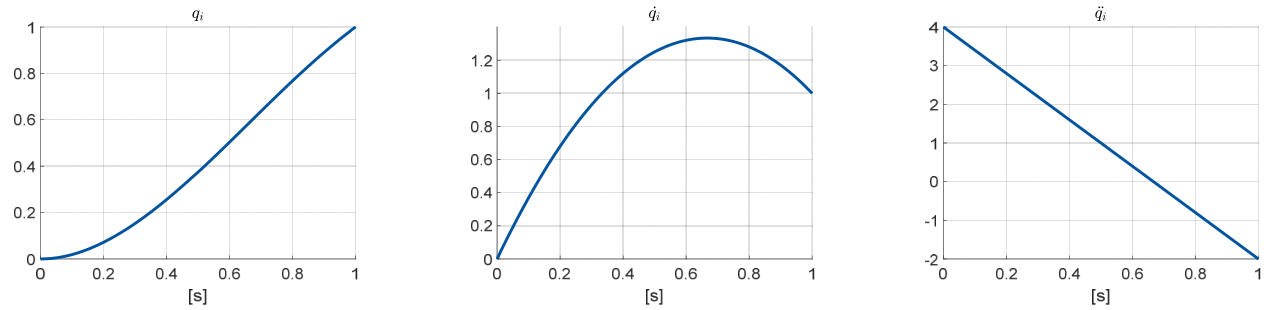
\includegraphics[width=\textwidth]{cubic-polynomial.png}
		\caption{Example of cubic polynomial.}
	\end{figure}
	\item Fifth order polynomial for the joints motion: allows imposing start, end positions, velocities and accelerations with finite jerk.
	\begin{align*}
		&q_i(t) = a_{i,5}t^5 + a_{i,4}t^4 + a_{i,3}t^3 + a_{i,2}t^2 + a_{i,1}t + a_{i,0} &&-\text{fifth order polynomial}\\
		&\dot{q}_i(t) = 5a_{i,5}t^4 + 4a_{i,4}t^3 + 3a_{i,3}t^2 + 2a_{i,2}t + a_{i,1} &&-\text{forth order velocity profile}\\
		&\ddot{q}_i(t) = 20a_{i,5}t^3 + 12a_{i,4}t^2 + 6a_{i,3}t + 2a_{i,2} &&-\text{cubic acceleration profile}
	\end{align*}
	\begin{figure}[hbt!]
		\centering
		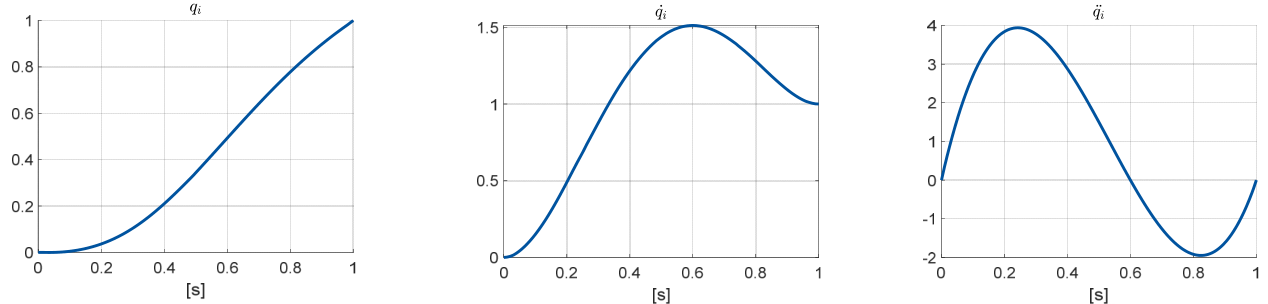
\includegraphics[width=\textwidth]{fifth-order-polynomial.png}
		\caption{Example of fifth order polynomial.}
	\end{figure}
	\item Trapezoidal acceleration profile: given time period, $\max$ acceleration, velocity and position.
	\note Just know that the below formulas and constraints exist. The derivation is complicated and time-consuming.
	\begin{align*}
		\Delta t_{i,I} &= T - \frac{\dot{q}_{\max}}{\ddot{q}_{\max}} - \frac{q_{\max}}{\dot{q}_{\max}} && \frac{q_{\max}}{T} \leq \dot{q}_{\max} \leq \frac{2q_{\max}}{T}\\
		\Delta t_{i,II} &= 2\frac{\dot{q}_{\max}}{\ddot{q}_{\max}} + \frac{q_{\max}}{\dot{q}_{\max}} -T && \frac{\dot{q}_{\max}}{T - \frac{q_{\max}}{\dot{q}_{\max}}} \leq \ddot{q}_{\max} \leq \frac{2\dot{q}_{\max}}{T - \frac{q_{\max}}{\dot{q}_{\max}}}\\
		\Delta t_{i,IV} &= T - 4 \Delta t_{i,I} - 2 \Delta t_{i,II} && \dddot{q}_{\max} = \frac{\ddot{q}_{\max}}{\Delta t_{i,I}} = \frac{\ddot{q}_{\max}}{T - \frac{\dot{q}_{\max}}{\ddot{q}_{\max}} - \frac{q_{\max}}{\dot{q}_{\max}}}\\
	\end{align*}
	\begin{figure}[hbt!]
		\centering
		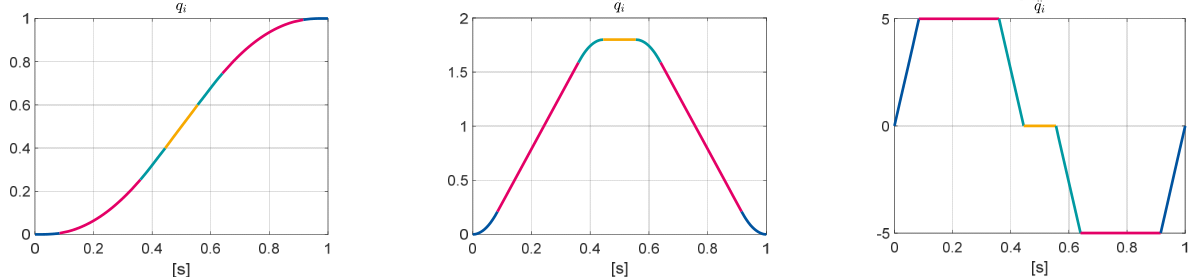
\includegraphics[width=\textwidth]{trapezoidal-acceleration-profile.png}
		\caption{Example of trapezoidal acceleration profile.}
	\end{figure}
\end{itemize}

\subsection{Motion through a Sequence of Points}
\begin{itemize}
	\item This can be viewed as extension of point-to-point motion
	\item The path is defined through a \textbf{sequence of $N$ path points}
	\item The time instances when these points must be reached should also be given
	\item Instead of using an $(N+3)$-order polynomial through $N$ joint configurations, we can use low-order interpolating polynomials (\figref{fig:interpolating-polynomials}).
	\begin{itemize}
		\item Each joint variable $q_i$ corresponds to a set of $N-1$ cubic polynomials $\Pi_{i,k}(t), k=1, \dots, N-1$
	\end{itemize}
	\begin{align*}
		q_i(t_k) &= q_{i,k} &&-\text{intermediate poses}\\
		q_{i,1} &= q_{i,start}, q_{i,N} = q_{i,end}\\
		t_{i,1} &= t_{i,start}, t_{i,N} = t_{i,end}\\
		\Pi_{i,k}(t_k) &= \Pi_{i,k+1}(t_k) = q_{i,k} &&-\text{path continuity}
	\end{align*}
	\item To impose \textbf{velocity continuity}, additional information is needed
	\[ \dot{\Pi}_{i,k}(t_{i,k+1}) = \dot{\Pi}_{i,k+1}(t_{i,k+1}) = \dot{q}_i(t_{i,k+1}) \]
	\begin{itemize}
		\item Arbitrary values for the velocity at the path points $\dot{q}_i(t_k)$ \textbf{or}
		\item Values for the velocity at the path points $\dot{q}_i(t_k)$ according to some criteria \textbf{or}
		\item Impose continuous acceleration at the path points
	\end{itemize}
	\note Probably leads to acceleration jerks
	\item Continuity for acceleration: imposed by 4 equations\\
	\note Required using 2 additional virtual points for 2 additional polynomials $\Rightarrow 4(N+1)$ equations for $4(N+1)$ unknowns. It is computationally expensive. With some tricks, the problem can be reduced to $N$ variables \dots
\end{itemize}

\begin{figure}[hbt!]
	\centering
	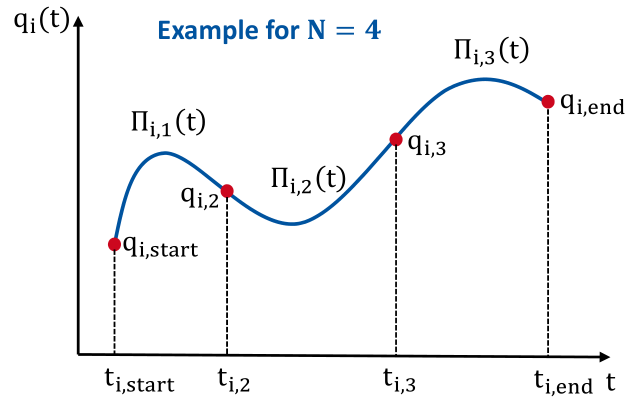
\includegraphics[width=0.5\textwidth]{interpolating-polynomials.png}
	\caption{Example of motion through sequence of four points using low-order (cubic) interpolating polynomials.}
	\label{fig:interpolating-polynomials}
\end{figure}

\section{Operational-space Trajectories}
\begin{itemize}
	\item Planning in the Joint Space may result in unexpected \ac{ee} motion, resulting from the non‐linear direct kinematics.
	\item Planning in Operational Space ensures that the \ac{ee} motion follows exactly the geometrically specified path by
	\begin{itemize}
		\item interpolating a sequence of prescribed poses
		\item generating analytical motion primitives (e.g. lines, circular arcs etc.)
		\item but it requires \hlr{real time} inverse kinematic computation, which is more computationally expensive
	\end{itemize}
	\item {\color{red}\boxed{\text{Path primitives + timing laws = trajectory planning}}}\\
	analyzed and computed separately
\end{itemize}

\subsection{Path primitive}
\begin{itemize}
	\item The word \textit{primitive} means a basic component, from which other is derived.
	\item \hlr{Path primitives} are the analytical geometrical descriptions for paths.
	\item Parametric representation of the path $\Gamma$ in space is a function of a general parameter $\sigma$ describe the position vector for point $\textbf{P}$ (\figref{fig:path-parametric-representation})
	\[ \textbf{r}_{\textbf{P}, \prescript{j}{}{O}} = \textbf{r}_\textbf{P} = \textbf{r}_\textbf{P}(\sigma), \quad \sigma\in[\sigma_{start}, \sigma_{end}]\]
	\item Usually it makes sense to replace general \ac{param} $\sigma$ by the current path length $s$
	\[ \textbf{r}_\textbf{P}(s) = f(s) \quad\text{with}\quad \sigma_{start}=0, \sigma_{end} = s_{end} \]
\end{itemize}

\begin{figure}[hbt!]
	\centering
	\begin{minipage}{0.45\textwidth}
		\centering
		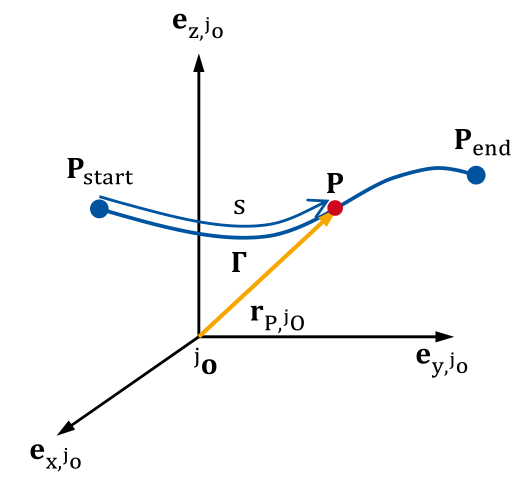
\includegraphics[width=\textwidth]{path-parametric-representation.png}
		\caption{Example for parametric representation of path $\Gamma$}
		\label{fig:path-parametric-representation}
	\end{minipage}\hfill
	\begin{minipage}{0.45\textwidth}
		\centering
		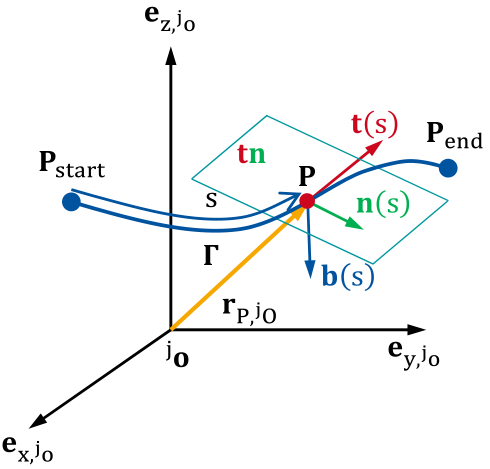
\includegraphics[width=\textwidth]{frenet-frame.png}
		\caption{Frenet frame with 3 unit vectors.}
		\label{fig:frenet-frame}
	\end{minipage}
\end{figure}

\subsection{Frenet Frame}
Frenet Frame is used to define the coordinate orientation along the path $\Gamma$. The three unit vectors establish the Frenet frame (\figref{fig:frenet-frame}):
\begin{itemize}
	\item Tangent unit vector $\displaystyle {\color{red} \textbf{t}(s)} = \frac{d\textbf{r}_P(s)}{ds} $ along the direction of the path
	\item Normal unit vector $\displaystyle {\color{Green} \textbf{n}(s)} = \frac{1}{\left|\left| \frac{d^2 \textbf{r}_P(s)}{ds^2} \right| \right|} \frac{d^2 \textbf{r}_P(s)}{ds^2} $ perpendicular to ${\color{red} \textbf{t}(s)}$
	\item Binormal unit vector $\displaystyle {\color{blue} \textbf{b}(s)} = {\color{red} \textbf{t}(s)} \times {\color{Green} \textbf{n}(s)}$ complements a right handed moving frame
\end{itemize}

\subsection{Path Primitive: Rectilinear Path}
The simplest parametric path representation is a linear segment between $\textbf{P}_{start}$ and $\textbf{P}_{end}$
\begin{align}
	\textbf{r}_{P,\prescript{j}{}{O}}(s) &= \textbf{r}_{P_{start}, \prescript{j}{}{O}} + \frac{s}{\left|\left| \textbf{r}_{P_{end}, \prescript{j}{}{O}} - \textbf{r}_{P_{start}, \prescript{j}{}{O}} \right|\right|} \left( \textbf{r}_{P_{end}, \prescript{j}{}{O}} - \textbf{r}_{P_{start}, \prescript{j}{}{O}} \right)\\
	{\color{red} \textbf{t}(s)} &= \frac{d\textbf{r}_P(s)}{ds} = \frac{1}{\left|\left| \textbf{r}_{P_{end}, \prescript{j}{}{O}} - \textbf{r}_{P_{start}, \prescript{j}{}{O}} \right|\right|} \left( \textbf{r}_{P_{end}, \prescript{j}{}{O}} - \textbf{r}_{P_{start}, \prescript{j}{}{O}} \right)\\
	{\color{Green} \textbf{n}(s)} &= \frac{1}{\left|\left| \frac{d^2 \textbf{r}_P(s)}{ds^2} \right| \right|} \frac{d^2 \textbf{r}_P(s)}{ds^2} \quad\text{with}\quad \frac{d^2 \textbf{r}_{P,\prescript{j}{}{O}}(s)}{ds^2}=0
\end{align}
$\Rightarrow$ \hlr{CAN NOT} define the Frenet frame uniquely. The plane ${\color{red}\textbf{t}\color{Green}\textbf{n}}$ can be rotated arbitrarily around ${\color{red} \textbf{t}(s)}$

\begin{figure}[hbt!]
	\centering
	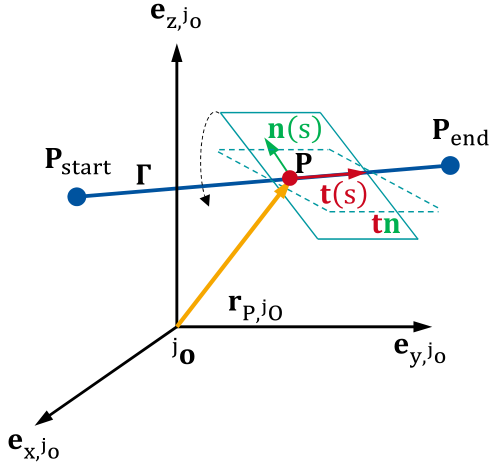
\includegraphics[width=0.3\textwidth]{rectilinear-path.png}
	\caption{Rectilinear path primitive.}
	\label{fig:rectilinear-path}
\end{figure}

\subsection{Path Primitive: Circular Arc}
The circular arc is defined through three points $\textbf{P}_{start}$, $\textbf{P}_{mid}$ and $\textbf{P}_{end}$.

\begin{minipage}{.5\textwidth}
	\begin{itemize}
		\item Compute center $\prescript{j}{}{\textbf{r}}_{\prescript{C}{}{O}, \prescript{j}{}{O}}$
		\begin{itemize}
			\item Determine $\prescript{j}{}{\textbf{r}}_{P_{mid}, P_{start}}$
			\item Determine $\prescript{j}{}{\textbf{r}}_{P_{end}, P_{start}}$
			\item Determine unit vector $\prescript{j}{}{\textbf{e}}_{z,\prescript{C}{}{O}}$
			\item Determine helper vectors $\textbf{r}_{H_1}, \textbf{r}_{H_2}$
			\item Determine $\prescript{j}{}{\textbf{r}}_{\prescript{C}{}{O}, \prescript{j}{}{O}}$
		\end{itemize}
		\item Determine unit vectors $\prescript{j}{}{\textbf{e}}_{x,\prescript{C}{}{O}}, \prescript{j}{}{\textbf{e}}_{y,\prescript{C}{}{O}}$
		\item Determine radius
		\item \dots
	\end{itemize}
\end{minipage}
\begin{minipage}{.45\textwidth}
	\centering
	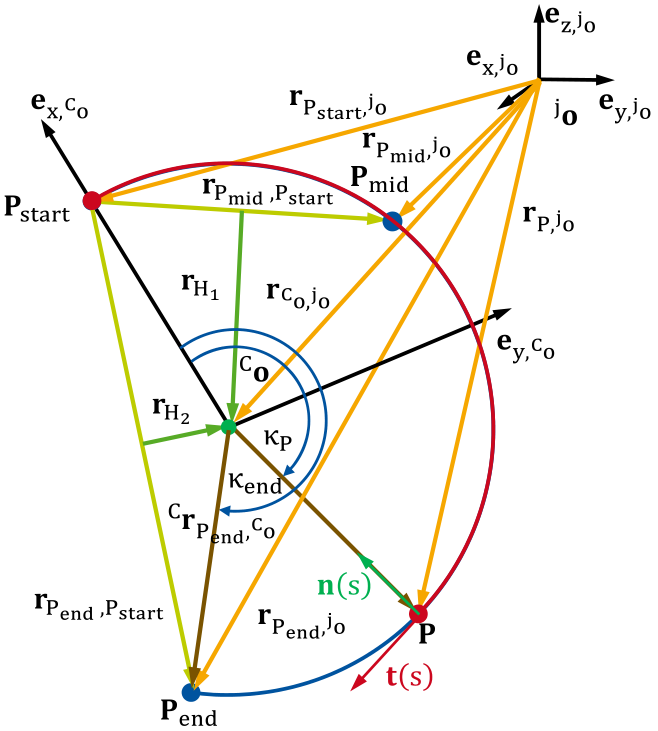
\includegraphics[width=\textwidth]{circular-arc.png}
\end{minipage}

\subsection{Path Primitive: Spline Path}
Given a set of points $\textbf{P}_i$ for $i\in\{1,n\}$, a smooth curves is generated by interpolating method
\begin{itemize}
	\item Between two consecutive points $\textbf{P}_i$ and $\textbf{P}_{i+1}$, there is path segment $\textbf{S}_i(\lambda)$
	\item To ensure smoothness between path's segments, the path must be continuous up to its second derivative at path points
	\item Use polynomials of degree five
	\[\textbf{S}_i(\lambda) = a_{i,5} \lambda^5 + a_{i,4} \lambda^4 + a_{i,3} \lambda^3 + a_{i,2} \lambda^2 + a_{i,1} \lambda + a_{i,0}, \qquad 0\leq \lambda \leq \lambda_i \]
\end{itemize}

\begin{figure}[hbt!]
	\centering
	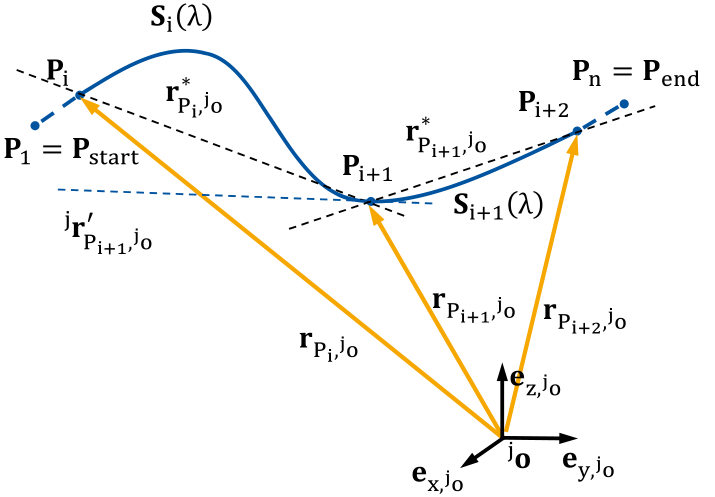
\includegraphics[width=0.5\textwidth]{spline-path.png}
	\caption{Spline path primitive.}
	\label{fig:spline-path}
\end{figure}

\section{Nonlinear Dynamics Motor Primitives}
This \textit{nonlinear dynamics motor primitives} are NOT the same as path primitives mentioned above. Let's examine two second-order dynamic systems $(z,y)$ and $(v,x)$ as follows: \cite{ijspeert2002movement}
\begin{align}
	\dot{z} &= f_z(y,z) = \alpha_z (\beta_z (g-y) - z)\\
	\dot{y} &= f_y(z,x,v) = z + \frac{\sum_{i=1}^N \Psi_i w_i}{\sum_{i=1}^N \Psi_i} v\\
	\dot{v} &= f_v(x,v) = \alpha_v (\beta_v (g-x) -v)\\
	\dot{x} &= f_x(v) = v\\
	\Psi_i &= \exp \left( -\frac{1}{2\sigma_i^2} (\tilde{x}-c_i)^2 \right), \quad i = 1, \dots, N &&-\text{Gaussian kernel functions}\\
	\tilde{x} &= \frac{x - x_0}{g - x_0}
\end{align}
\begin{itemize}
	\item The 2nd system dynamic behavior is simply analogous to value tracking: variable $x$ goes to target value $g$, the velocity $v$ starts and ends at 0 (\figref{fig:trajectory-tracking-1}).
	\item Compared to the 2nd one, the 1st system is just different in the extra nonlinear term in $\dot{y}$
	\item This is similar as with Fourier series. Fourier series is used to approximate an arbitrary time series data via a weighted sum of multiple sinusoidal functions. Here, we approximate the different between the velocity profile for trajectory tracking and for value tracking by a weighted sum of Gaussian-like functions.
	\item The above dynamical system is spatially invariant in the sense that scaling of the goal $g$ does not affect the topology of the attractor landscape
\end{itemize}

\begin{figure}[hbt!]
	\centering
	\begin{minipage}{0.49\textwidth}
		\centering
		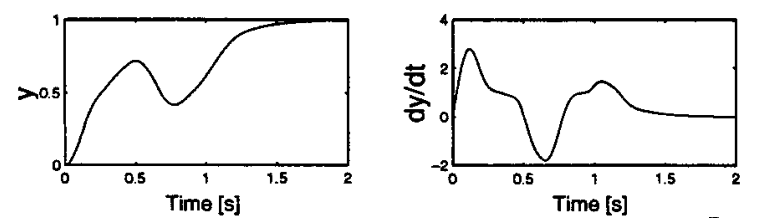
\includegraphics[width=\textwidth]{trajectory-tracking.png}
		\caption{Trajectory tracking: $y$ as joint position and velocity profile $\dot{y}$.}
		\label{fig:trajectory-tracking}
	\end{minipage}\hfill
	\begin{minipage}{0.49\textwidth}
		\centering
		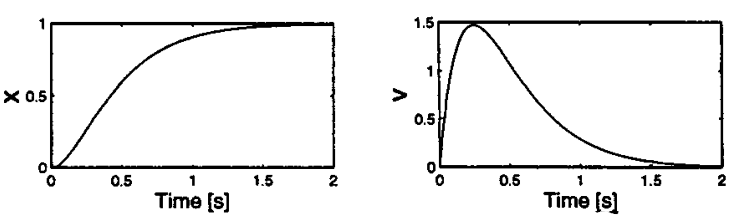
\includegraphics[width=\textwidth]{trajectory-tracking-1.png}
		\caption{Value tracking: $x$ as joint position and velocity profile $\dot{x}$.}
		\label{fig:trajectory-tracking-1}
	\end{minipage}
	\begin{minipage}{0.4\textwidth}
		\centering
		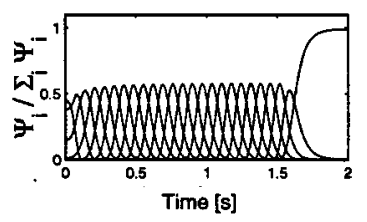
\includegraphics[width=\textwidth]{trajectory-tracking-2.png}
		\caption{Basis functions from Gaussian kernels.}
		\label{fig:trajectory-tracking-2}
	\end{minipage}
\end{figure}

With regards to trajectory planning, long story short, we manage to parameterize a trajectory $y$ to \ac{param} $w_i$
\begin{itemize}
	\item $q$ - current joint position
	\item $g$ - desired joint position
	\item $x$ - a timing signal
	\item $v$ - a scaling signal
\end{itemize}

Given a new trajectory:
\begin{itemize}
	\item Shift the given trajectory to $0$ start position
	\item Scale the time constants of the dynamical system such that $(v,x)$ reaches $(0,g)$ at approximately the same time $\Rightarrow$ a time trajectory for $v(t),x(t)$
	\item Given $v(t),x(t)$, calculate $u_{des} = \dot{y}_{demo} - z$ as desired output
	\item Learn $w_i$ via recursive least squares to minimize the locally weighted error criterion for each local model $u_{i,t} = w_i v_t$
	\[J_i = \sum_t \Psi_{i,t} (u_{des,t} - u_{i,t})^2\]
\end{itemize}

This parameterization approach satisfies following requirements: 
\begin{itemize}
	\item Able to fit a demonstrated trajectories with high precision (fitting all \ac{dof} and all points of the trajectories)
	\item Able to generate similar movements to different goals. If we fix the weights $w_i$, change the goal $g$, we will receive a similar trajectories. \note good with close targets, better with variation in height, not with left and right.
	\item Robust against perturbations (\eg, in scenarios there is interaction with external objects)
	\begin{align}
		&\tilde{y} &&-\text{the actual position}\\
		&\dot{y} = \alpha_y \left( \frac{\sum_{i=1}^N \Psi_i, w_i}{\sum_{i=1}^N \Psi_i} v + z \right) + \alpha_{py} (\tilde{y} - y)\\
		&\dot{x} = v \left( 1+ \alpha_{px}(\tilde{y}-y)^2 \right) ^{-1}
	\end{align}
	\item Good basis for comparing movements, as a metric for measuring differences between movements. Similar movements will have similar weights $w_i$ $\Rightarrow$ can be used to classify movements (simple nearest neighbors)
\end{itemize}

\todo{The effect of hyper-\ac{param}}
\begin{itemize}
	\item $\alpha_v$
	\item $\beta_v$
	\item $\alpha_z$
	\item $\beta_z$
	\item $c_i$
	\item \dots
\end{itemize}